
\subsection{Kinematik}

\subsubsection{Aufgaben}
Die Kinematik dient als Grundstein für die Pfadberechnung erfüllt zwei elementare Aufgaben. Mit Hilfe der direkten Kinematik kann, bei gegebenen Winkelstellungen und Achsenlängen, die aktuelle Position des Werkzeugs im Koordinatensystem berechnet werden. Für die Interpolation von wesentlich größerer Bedeutung, ist jedoch die inverse Kinematik mit welcher die Winkelstellungen der Achsen, bei gegebenen Zielpunkt und Achsenlängen, berechnet werden können.

\subsubsection{Aufbau}
Die Verfahren zur direkten beziehungsweise indirekten Kinematik sind in der Klasse Kinematics als statische Methoden CalculateDirect und CalculateInverse implementiert. Da diese Methoden unabhängig von der API arbeiten, können sie universell angewendet werden. So könnten sie beispielsweise auch in der Spieleentwicklung zur Animation von Grafiken verwendet werden.

\subsubsection{Umsetzung}
\textbf{Kinematics}\\
Die im Aufbau erwähnten Methoden der Kinematics-Klasse sind wie folgt implementiert:
\begin{itemize}
\item \textbf{CalculateDirect}\\
Bei Aufruf dieser Methode wird mit dem Verfahren der direkten Kinematik und den angegebenen Parametern die Position des Werkzeugs, bei gegebenen Winkelstellungen und Achsenlängen berechnet. Als Parameter werden ihr die Winkelstellungen der ersten Achse $\alpha_1$ und der zeiten Achse $\alpha_2$, sowie die Länge der ersten und zweiten Achse, $l_1$ und $l_2$, als float-Werte übergeben. Mit diesen Informationen kann nun berechnet werden an welchem Punkt sich das Werkzeug im Koordinatensystem befindet.\\
\begin{figure}[H]
  \centering
  \begin{minipage}[t]{12 cm}
  	\centering
  	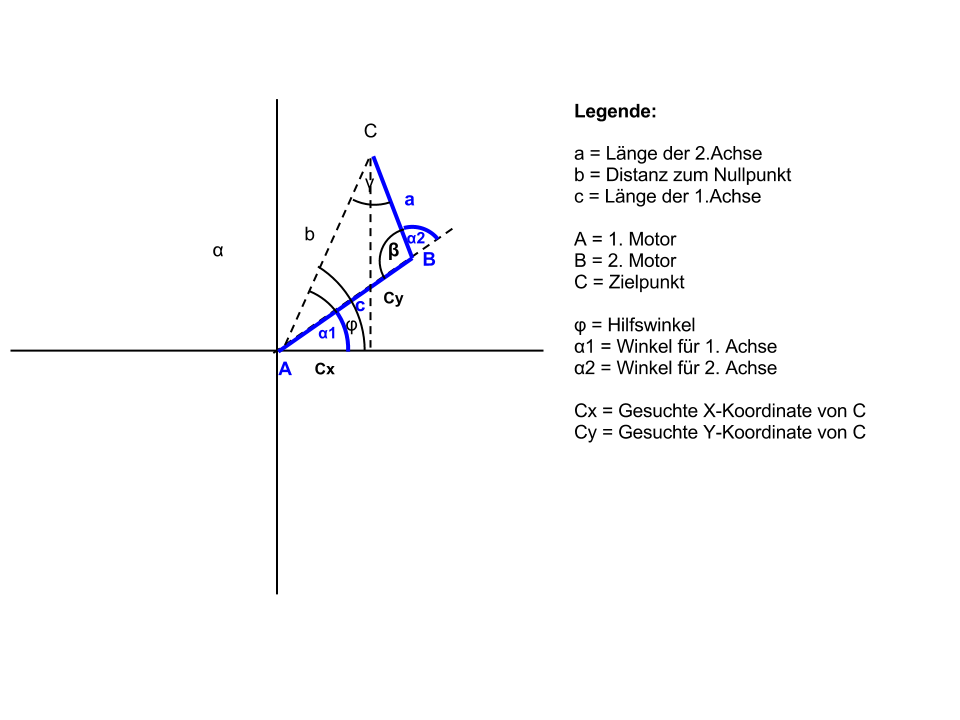
\includegraphics[width=12cm]{images/Direktkinematik} 
    \caption{Skizze zur direkten Kinematik}
  \end{minipage}
\end{figure}
Der Punkt wird nach folgendem Schema berechnet:
\begin{enumerate}
\item Berechnung des Winkels $\beta$\\
Der Winkel $\beta$ kann bei gegebenenen $\alpha_2$ relativ einfach berechnet werden (siehe Skizze) und ist nötig um anschließend die Distanz $d$ zu berechnen\\
\begin{align*}
\beta = 180^\circ - \alpha_2
\end{align*}
\item Berechnung der Distanz $d$\\
Um $d$ zu berechnen wird der Kosinussatz für $\beta$ verwendet:
\begin{align*}
b^2 = a^2+c^2-2ac\cos\beta \\
b = \sqrt{a^2+c^2-2ac\cos\beta}
\end{align*}
Angepasst an unsere Variablen entsteht daraus die Formel:
\begin{align*}
d = \sqrt{l_1^2+l_2^2-2l_1l_2\cos\beta}
\end{align*}
\item Berechnung des Winkels $\alpha$\\
Um zu den gesuchten Koordinaten zu gelangen benötigen wir den Referenzwinkel $\varphi$, welcher aus der Summe von $\alpha$ und $\alpha1$ definiert ist. Der Winkel $\alpha$ kann über die Umformung des Kosinussatzes berechnet werden:
\begin{align*}
a^2 & = b^2 + c^2 - 2bc \cos \alpha \\
2bc \cos \alpha & = b^2 + c^2 - a^2 \\
\cos \alpha & = \frac{b^2 + c^2 - a^2}{2bc} \\
\alpha & = \arccos \frac{b^2 + c^2 - a^2}{2bc}
\end{align*}
Angepasst an unsere Variablen entsteht daraus die Formel:
\begin{align*}
\alpha = \arccos \frac{d^2 + l_1^2 - l_2^2}{2dl_1}
\end{align*}
\item Berechnung des Referenzwinkels $\varphi$\\:
\begin{align*}
\varphi = \alpha + \alpha_1
\end{align*}
\item Berechnung des gesuchten Punkts\\
Mit dem nun vorhandenen Zahlenmaterial kann nun der gesuchte Punkte über die Sinus beziehungsweise Kosinus-Funktion im rechtwinkeligen Dreieck berechnet werden.
\begin{align*}
x &= d * \cos \varphi \\
y &= d * \sin \varphi
\end{align*}
\end{enumerate}
\item \textbf{CalcualteInverse}\\
Bei Aufruf dieser Methode wird mit dem Verfahren der inversen Kinematik und den angegebenen Parametern ein Winkelstellungen der Achsen am angegeben Zielpunkt berechnet. Als Parameter werden ihr der Zielpunkt als Point3D-Objekt, sowie die Länge der ersten zweiten Achse als float-Wert übergeben. Mit diesen Informationen kann nun berechnet werden welchen Winkel die Achsen einnehmen müssen, damit  sich der Werkzeugmittelpunkt am Zielpunkt befindet.\\
\begin{figure}[H]
  \centering
  \begin{minipage}[t]{12 cm}
  	\centering
  	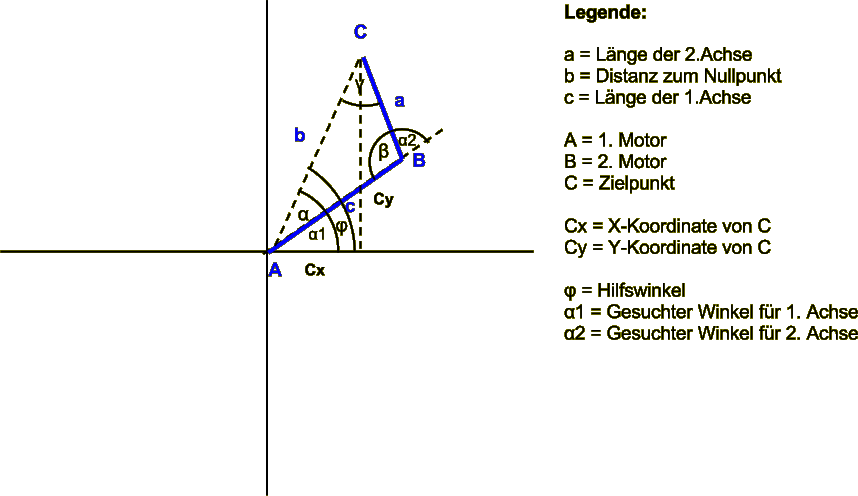
\includegraphics[width=12cm]{images/Inverskinematik} 
    \caption{Skizze zur inversen Kinematik}
  \end{minipage}
\end{figure}
Die Berechnung der Winkel läuft nach folgendem Schema ab:
\begin{enumerate}
\item Deklarieren der Hilfsvariablen\\
Zur Vereinfachung der Berechnung werden zuerst die Variablen $x$,$y$,$z$ vom Typ float definiert. Diesen Variablen werden entsprechend die X-,Y- und Z-Koordinaten des Zielpunkts zugewiesen.
\item Berechnung der Distanz $d$\\
Zur Berechnung der Winkel werden die Seitenlängen des allgemeinen Dreiecks, welches durch die beiden Achsen $l_1$ und $l_2$ sowie die Distanz zum Zielpunkt $d$ gebildet wird, benötigt. Da die Längen der Achsen bereits bekannt sind, muss nur die Distanz d durch Verwendung des Satzes des Pythagoras zusammen mit den x- und y-Koordinaten berechnet werden.\\
\begin{equation*}
d = \sqrt{x^2 + y^2}
\end{equation*}
\item Auf Spezialfall prüfen\\
Als Spezialfall wird in diesem Kontext ein vollkommen ausgestreckter Roboterarm am Zielpunkt betrachtet. Da bei dieser Konstellation kein Dreieck entsteht, können die Winkel nicht auf herkömmlichen Weg berechnet werden. In diesem Fall können die Winkel jedoch durch logische Überlegung bestimmt werden, da der Winkel der zweiten Achse $\alpha_2$ dabei immer 0$^\circ$ beträgt.\\
Die Winkelstellung der ersten Achs $\alpha_1$ e kann durch die x- und y-Koordinate folgendermaßen bestimmt werden.
\begin{align*}
x & = l_1+l_2 &\wedge && y & = 0 & \alpha_1 & = 0^\circ \\
x & = -(l_1+l_2) &\wedge && y & = 0 & \alpha_1 & = 180^\circ \\ 
x & = 0 &\wedge && y & = l_1+l_2 & \alpha_1 & = 90^\circ \\
x & = 0 &\wedge && y & = -(l_1+l_2) & \alpha_1 & = 270^\circ
\end{align*}
Da nun beide Winkel bestimmt sind, wird ein InterpolationStep mit den soeben berechneten Werten erzeugt und zurückgegeben.
\item Berechnung der Innenwinkel\\
Da nun alle drei Seitenlängen bekannt sind, können die Innenwinkel $\alpha$, $\beta$, $\gamma$ über den Kosinussatz berechnet werden.\\
\\
Umformung des Kosinussatzes für $\alpha$:
\begin{align*}
a^2 & = b^2 + c^2 - 2bc \cos \alpha \\
2bc \cos \alpha & = b^2 + c^2 - a^2 \\
\cos \alpha & = \frac{b^2 + c^2 - a^2}{2bc} \\
\alpha & = \arccos \frac{b^2 + c^2 - a^2}{2bc}
\end{align*}
Umformung des Kosinussatzes für $\beta$:
\begin{align*}
b^2 & = a^2 + c^2 - 2ac \cos \beta \\
2ac \cos \beta & = a^2 + c^2 - b^2 \\
\cos \beta & = \frac{a^2 + c^2 - b^2}{2ac} \\
\beta & = \arccos \frac{a^2 + c^2 - b^2}{2ac}
\end{align*}
Umformung des Kosinussatzes für $\gamma$:
\begin{align*}
c^2 = a^2 + b^2 - 2ab \cos \gamma \\
2ab \cos \gamma = a^2 + b^2 - c^2 \\
\cos \gamma = \frac{a^2 + b^2 - c^2}{2ab} \\
\gamma = \arccos \frac{a^2 + b^2 - c^2}{2ab}
\end{align*}
Auf unsere Variablen angepasst sehen die Formeln für die Berechnung der Winkel folgendermaßen aus:
\begin{align*}
\alpha = \arccos \frac{d^2 + l_1^2 - l_2^2}{2dl_1} \\
\beta = \arccos \frac{l_2^2 + l_1^2 - d^2}{2l_1l_2} \\
\gamma = \arccos \frac{d^2 + l_2^2 - l_1^2}{2dl_2}
\end{align*}
\item Berechnung des Referenzwinkels $\varphi$:\\
Im nächsten Schritt wird noch der Referenzwinkel $\varphi$, welcher die Position des Dreiecks im Koordinatensystem festlegt, berechnet. Dieser Winkel befindet sich in einem rechtwinkeligen Dreieck, welches durch $d$, $x$ und $y$ definiert wird und kann durch Umformung der Sinusfunktion im rechtwinkeligen Dreieck berechnet werden:
\begin{align*}
\varphi = \arccos \frac{x}{d}
\end{align*}
\item Überprüfen des Quadranten:\\
Da die Arkussinus-Funktion lediglich einen Winkel zwischen 0$^\circ$ und 180$^\circ$ liefert, muss der Quadrant in dem sich der Zielpunkt befindet überprüft werden. Befindet sich dieser im 3. oder 4. Quadranten, so wird das Vorzeichen des Referenzwinkels $\varphi$ umgedreht. Alternativ könnte man auch 180$^\circ$ zum Referenzwinkel addieren.
\item Berechnung von $\alpha_1$ und $\alpha_2$\\
Mit dem nun vorhandenen Zahlenmaterial können die gesuchten Winkel der ersten und zweiten Achse folgendermaßen berechnet werden:
\begin{itemize}
\item Berechnung von $\alpha_1$:\\
Der Winkel der ersten Achse ergibt sich aus der Differenz zwischen dem Referenzwinkel $\varphi$ und dem Innenwinkel $\alpha$
\begin{align*}
\alpha_1 = \varphi - \alpha
\end{align*}
\item Berechnung von $\alpha_2$:\\
Der Winkel der zweiten Achse ergibt sich aus der Differenz zwischen 180$^\circ$ und dem Innenwinkel $\beta$
\begin{align*}
\alpha_2 = 180 - \beta
\end{align*}
\end{itemize}

\end{enumerate}
\end{itemize}